\documentclass{article}

\usepackage[utf8]{inputenc}

\usepackage{nicefrac}
\usepackage{amssymb, amsmath, amsfonts}
\usepackage{amsthm}
\usepackage{tikz}
\usetikzlibrary{matrix,shapes,arrows}
\usepackage{pgfplots}
\usepgfplotslibrary{groupplots}
\usepackage[a4paper, margin=1in]{geometry}

\newtheorem{proposition}{Proposition}
\newtheorem{theorem}{Theorem}
\newtheorem{definition}{Definition}
\newtheorem{lemma}{Lemma}
\newtheorem{conjecture}{Conjecture}
\newtheorem{corollary}{Corollary}
\newtheorem{remark}{Remark}
\newtheorem{assumption}{Assumption}

\newlength\figureheight
\newlength\figurewidth
\setlength\figureheight{12cm}
\setlength\figurewidth{14cm}

\newcommand{\tikzdir}[1]{tikz/#1.tikz}
\newcommand{\inputtikz}[1]{\input{\tikzdir{#1}}}

\DeclareMathOperator*{\argmin}{arg\; min}     % argmin
\DeclareMathOperator*{\argmax}{arg\; max}     % argmax
\DeclareMathOperator*{\tr}{tr}     % trace
\DeclareMathOperator{\Cov}{Cov}
\DeclareMathOperator{\logdet}{log\;det}

\title{EE3011 Modeling and Control\\Tutorial 11: Relative Stability/Lead Compensator}
\date{}
\begin{document} \maketitle
\begin{enumerate}
\item A feedback control system is as shown in Figure~\ref{fig:1}:

  \begin{figure}[h]
    \centering
    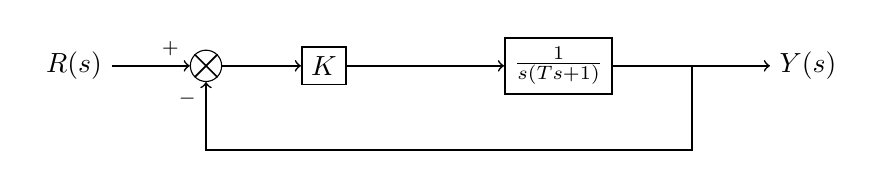
\begin{tikzpicture}
      \tikzstyle{point} = [coordinate]
      \tikzstyle{box} = [rectangle, draw, semithick]
      \matrix[row sep = 7mm, column sep = 10mm]{
        % first row
        \node (p1) [] {$R(s)$};&
        \node (p2) [circle,draw,inner sep=4pt] {};&
        \node (outer) [box] {$K$};&
        \node (p3) [point] {};&
        \node (inner) [box] {$\frac{1}{s(Ts+1)}$};&
        \node (p5) [point] {};&
        \node (p6) [] {$Y(s)$};\\
        % third row
        &
        \node (p9) [point] {};&
        &
        &
        &
        \node (p10) [point] {};&
        \\
      };
      \draw [semithick,->] (p1)--node[near end, above]{\scriptsize{$+$}} (p2);
      \draw [semithick,->] (p2)--(outer);
      \draw [semithick,->] (outer)--(p3)--(inner);
      \draw [semithick,->] (inner)--(p5)--(p6);
      \draw [semithick,->] (p5)--(p10)--(p9)--node[near end, left]{\scriptsize{$-$}} (p2);
      \draw [semithick] (p2.north east)--(p2.south west);
      \draw [semithick] (p2.south east)--(p2.north west);
    \end{tikzpicture}
    \caption{Block Diagram\label{fig:1}}
  \end{figure}
  Given that the phase margin of the system is $45^\circ$ and the gain crossover frequency is $3$rad/s, find the controller gain $K$ and the time constant $T$. Can you find a suitable value of gain $K$ in order to achieve a velocity error constant of no less than $5$ and a phase margin of no less than $45^\circ$ for the system?
\item A synchronous generator excitation control system is shown in Figure~\ref{fig:2}. 
  \begin{figure}[h]
    \centering
    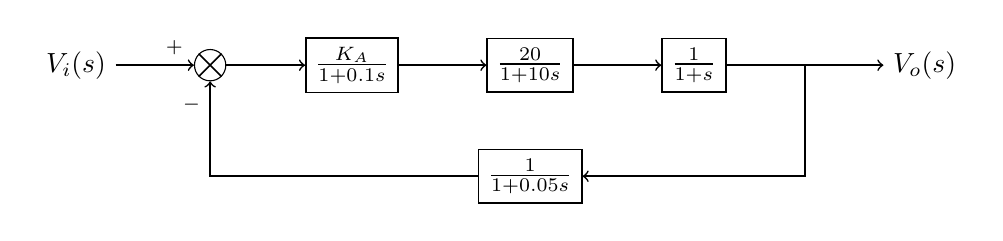
\begin{tikzpicture}
      \tikzstyle{point} = [coordinate]
      \tikzstyle{box} = [rectangle, draw, semithick]
      \matrix[row sep = 7mm, column sep = 10mm]{
        % first row
        \node (p1) [] {$V_i(s)$};&
        \node (p2) [circle,draw,inner sep=4pt] {};&
        \node (amp) [box] {$\frac{K_A}{1+0.1s}$};&
        \node (ex) [box] {$\frac{20}{1+10s}$};&
        \node (alt) [box] {$\frac{1}{1+s}$};&
        \node (p5) [point] {};&
        \node (p6) [] {$V_o(s)$};\\
        % third row
        &
        \node (p9) [point] {};&
        &
        \node (feed) [box] {$\frac{1}{1+0.05s}$};&
        &
        \node (p10) [point] {};&
        \\
      };
      \draw [semithick,->] (p1)--node[near end, above]{\scriptsize{$+$}} (p2);
      \draw [semithick,->] (p2)--(amp);
      \draw [semithick,->] (amp)--(ex);
      \draw [semithick,->] (ex)--(alt);
      \draw [semithick,->] (alt)--(p5)--(p6);
      \draw [semithick,->] (p5)--(p10)--(feed);
      \draw [semithick,->] (feed)--(p9)--node[near end, left]{\scriptsize{$-$}} (p2);
      \draw [semithick] (p2.north east)--(p2.south west);
      \draw [semithick] (p2.south east)--(p2.north west);
    \end{tikzpicture}
    \caption{Block Diagram\label{fig:2}}
  \end{figure}
\begin{enumerate}
\item The Bode plots of the open-loop transfer function with $K_A = 40$ are given in Figure~\ref{fig:3}. Determine the gain and phase margins of the system. Is the system stable?
\item By reducing the amplifier gain $K_A$, it is possible to improve the phase margin of the system. If the system is required to have a phase margin of $10^\circ$ , what should be the $K_A$?
\end{enumerate}
\item The frequency response of an industrial process is shown in Figure~\ref{fig:4}. Design a lead compensator that will yield a cross frequency of $10$rad/s and a phase margin of $50^\circ$.
\end{enumerate}

  \begin{figure}[t]
    \centering
    \inputtikz{Tut111}
    \caption{Bode plot of the synchronous generator\label{fig:3}}
  \end{figure}

  \begin{figure}[t]
    \centering
    \inputtikz{Tut112}
    \caption{Bode plot of an industrial process\label{fig:4}}
  \end{figure}
\end{document}
%%% Local Variables:
%%% TeX-command-default: "Latexmk"
%%% End:
